\documentclass[12pt,]{book}
\usepackage{lmodern}
\usepackage{amssymb,amsmath}
\usepackage{ifxetex,ifluatex}
\usepackage{fixltx2e} % provides \textsubscript
\ifnum 0\ifxetex 1\fi\ifluatex 1\fi=0 % if pdftex
  \usepackage[T1]{fontenc}
  \usepackage[utf8]{inputenc}
\else % if luatex or xelatex
  \ifxetex
    \usepackage{mathspec}
  \else
    \usepackage{fontspec}
  \fi
  \defaultfontfeatures{Ligatures=TeX,Scale=MatchLowercase}
\fi
% use upquote if available, for straight quotes in verbatim environments
\IfFileExists{upquote.sty}{\usepackage{upquote}}{}
% use microtype if available
\IfFileExists{microtype.sty}{%
\usepackage{microtype}
\UseMicrotypeSet[protrusion]{basicmath} % disable protrusion for tt fonts
}{}
\usepackage[margin=1in]{geometry}
\usepackage{hyperref}
\hypersetup{unicode=true,
            pdftitle={Challenges and Tools in the Assessment and Management of Pacific Salmon Fisheries},
            pdfauthor={Ben Staton},
            pdfborder={0 0 0},
            breaklinks=true}
\urlstyle{same}  % don't use monospace font for urls
\usepackage{natbib}
\bibliographystyle{myapalike}
\usepackage{longtable,booktabs}
\usepackage{graphicx,grffile}
\makeatletter
\def\maxwidth{\ifdim\Gin@nat@width>\linewidth\linewidth\else\Gin@nat@width\fi}
\def\maxheight{\ifdim\Gin@nat@height>\textheight\textheight\else\Gin@nat@height\fi}
\makeatother
% Scale images if necessary, so that they will not overflow the page
% margins by default, and it is still possible to overwrite the defaults
% using explicit options in \includegraphics[width, height, ...]{}
\setkeys{Gin}{width=\maxwidth,height=\maxheight,keepaspectratio}
\IfFileExists{parskip.sty}{%
\usepackage{parskip}
}{% else
\setlength{\parindent}{0pt}
\setlength{\parskip}{6pt plus 2pt minus 1pt}
}
\setlength{\emergencystretch}{3em}  % prevent overfull lines
\providecommand{\tightlist}{%
  \setlength{\itemsep}{0pt}\setlength{\parskip}{0pt}}
\setcounter{secnumdepth}{5}
% Redefines (sub)paragraphs to behave more like sections
\ifx\paragraph\undefined\else
\let\oldparagraph\paragraph
\renewcommand{\paragraph}[1]{\oldparagraph{#1}\mbox{}}
\fi
\ifx\subparagraph\undefined\else
\let\oldsubparagraph\subparagraph
\renewcommand{\subparagraph}[1]{\oldsubparagraph{#1}\mbox{}}
\fi

%%% Use protect on footnotes to avoid problems with footnotes in titles
\let\rmarkdownfootnote\footnote%
\def\footnote{\protect\rmarkdownfootnote}

%%% Change title format to be more compact
\usepackage{titling}

% Create subtitle command for use in maketitle
\newcommand{\subtitle}[1]{
  \posttitle{
    \begin{center}\large#1\end{center}
    }
}

\setlength{\droptitle}{-2em}

  \title{Challenges and Tools in the Assessment and Management of Pacific Salmon
Fisheries}
    \pretitle{\vspace{\droptitle}\centering\huge}
  \posttitle{\par}
    \author{Ben Staton}
    \preauthor{\centering\large\emph}
  \postauthor{\par}
    \date{}
    \predate{}\postdate{}
  
\usepackage{booktabs}
%%% This is an example file for the Auburn University style options
%%%       aums.sty (Masters Thesis)
%%%       auphd.sty (Ph.D. Dissertation)
%%%       auhonors.sty (Honors Scholar)

%%%To use it, please edit the necessary options, title, author, date, year, keywords, advisor, professor, etc. 

% \documentclass[12pt]{report}
\usepackage{setspace}
% \usepackage{titlesec}
%\setcounter{secnumdepth}{3}
% \usepackage{aums}       % For Master's papers
\usepackage{auphd}     % For Ph.D.
%\usepackage{auhonors}  % For honors college
\usepackage[normalem]{ulem}       % underlining on style-page; see \normalem below
\usepackage{url}
\usepackage[table]{xcolor}
\usepackage{tikz}
\usepackage{pgf}
\usepackage{color,soul}
\usepackage{float}
\usepackage{caption}
\captionsetup{width=\textwidth}

\usepackage{amsmath,amsthm, amsfonts, mathrsfs, graphicx, setspace, fullpage, color}
\usepackage{natbib, appendix}
\usepackage[T1]{fontenc}
\usepackage{multirow}
\usepackage{mathabx}
\RequirePackage{adjustbox}
% \usepackage{epstopdf}
\AtBeginDocument{\renewcommand{\bibname}{References}}
\usepackage{hyperref}
%\usepackage{tocloft}
%\renewcommand\cftchapafterpnum{\vskip\baselineskip}
%\renewcommand\cftsecafterpnum{\vskip\baselineskip}
%\renewcommand\cftsubsecafterpnum{\vskip\baselineskip}
%\renewcommand\cftsubsubsecafterpnum{\vskip\baselineskip}
%\renewcommand\cftfigafterpnum{\vskip\baselineskip}
%\renewcommand\cfttabafterpnum{\vskip\baselineskip}

% remove double spacing from itemized lists
\usepackage{enumitem}
% \setlist[itemize]{noitemsep}
\setlist{before=\doublespacing,after=\doublespacing}

% citation style: remove the comma between author and year 
\setcitestyle{aysep={}}
% \setlength{\bibhang}{2em}

%%%%%Format rules: Normal margins are 1 in. If you need to print with 1.5in margins, uncomment the line below
%\oddsidemargin0.5in \textwidth6in

%% If you do not need a List of Abbreviations, then comment out the lines below and the \printnomenclature line.
%%for List of Abbreviations information:  (see http://www.mackichan.com/TECHTALK/509.htm  )
% \usepackage[intoc]{nomencl}
% \renewcommand{\nomname}{List of Abbreviations}   	       
% \makenomenclature 
%% don't forget to run:   makeindex ausample.nlo -s nomencl.ist -o ausample.nls
%% Also, if 

\makeatother
\let\oldmaketitle\maketitle
\AtBeginDocument{\let\maketitle\relax}

% Put the title, author, and date in. 
\title{Challenges and Tools in the Assessment and Management of Pacific Salmon Fisheries}
\author{Benjamin A. Staton} 
\date{May 5, 2019} %date of graduation
\copyrightyear{2019} %copyright year

\keywords{Fisheries management, Bayesian inference, decision analysis}

% Put the Thesis Adviser here. 
\adviser{Matthew J. Catalano}

% Put the committee here (including the adviser), one \professor for each. 
% The advisor must be first, and the dean of the graduate school must be last.
\professor{Matthew J. Catalano, \textit{PLEASE INDICATE YOUR AFFILIATION}}

\professor{Asheber Abebe, \textit{PLEASE INDICATE YOUR AFFILIATION}}

\professor{Lewis G. Coggins, Jr., \textit{PLEASE INDICATE YOUR AFFILIATION}}

\professor{Conor P. McGowan, \textit{PLEASE INDICATE YOUR AFFILIATION}}
\usepackage{booktabs}
\usepackage{longtable}
\usepackage{array}
\usepackage{multirow}
\usepackage[table]{xcolor}
\usepackage{wrapfig}
\usepackage{float}
\usepackage{colortbl}
\usepackage{pdflscape}
\usepackage{tabu}
\usepackage{threeparttable}
\usepackage{threeparttablex}
\usepackage[normalem]{ulem}
\usepackage{makecell}

\usepackage{amsthm}
\newtheorem{theorem}{Theorem}[chapter]
\newtheorem{lemma}{Lemma}[chapter]
\theoremstyle{definition}
\newtheorem{definition}{Definition}[chapter]
\newtheorem{corollary}{Corollary}[chapter]
\newtheorem{proposition}{Proposition}[chapter]
\theoremstyle{definition}
\newtheorem{example}{Example}[chapter]
\theoremstyle{definition}
\newtheorem{exercise}{Exercise}[chapter]
\theoremstyle{remark}
\newtheorem*{remark}{Remark}
\newtheorem*{solution}{Solution}
\begin{document}
\maketitle

\begin{romanpages}      % roman-numbered pages 

\TitlePage 

\doublespacing
\setlength{\parskip}{0pt plus 0pt minus 0pt}

\begin{abstract} 
\noindent
I'm going to write an abstract to go here. This paragraph will be a brief introduction chapter 1: the overall topic of the research

This is the second paragraph of the dissertation abstract, which will talk broadly about chapter 2: run timing forecast models.

This is the second paragraph of the dissertation abstract, which will talk broadly about chapter 3: in-season MSE models.

This is the third paragraph of the dissertation abstract, which will talk broadly about chapter 4: multi-stock population dynamics models and the best ways to inform management trade-offs. 

\end{abstract}

\begin{acknowledgments}
\noindent
Here is where I will thank everyone:

Catalano, Coggins, Connors, Jones, Dobson, Farmer, Fleischman, Smith, Liller, Esquible, Bechtol, Spaeder, Decossas, AL-HPC folks, Auburn Hopper HPC folks. Folks at the lab. Family and Michelle. RStudio staff. Instructors: Abebe (complex quant problems), Stevison (Shell/bash/HPC), McGowan (SDM), Sawant (GIS).  

\end{acknowledgments}

\begin{singlespace}
	\tableofcontents
	\clearpage
	\listoffigures
	\clearpage
	\listoftables
\end{singlespace}

% \printnomenclature[0.5in] %used for the List of Abbreviations
\end{romanpages}        % All done with roman-numbered pages

\normalem       % Make italics the default for \em

% \titlespacing\section{0pt}{12pt plus 4pt minus 2pt}{0pt plus 2pt minus 2pt}
% \titlespacing\subsection{0pt}{12pt plus 4pt minus 2pt}{0pt plus 2pt minus 2pt}
% \titlespacing\subsubsection{0pt}{12pt plus 4pt minus 2pt}{0pt plus 2pt minus 2pt}

\setlength{\parskip}{0pt plus 0pt minus 0pt}

\doublespacing

\chapter{Evaluation of Intra-Annual Harvest Control Rules via
Closed-Loop Simulation}\label{ch3}

\section{Introduction}\label{introduction}

Here's chapter 3. It's about in-season simulation models for management
strategy evaluations.

\section{Methods}\label{methods}

I did some stuff.

\section{Results}\label{results}

I found some stuff.

\section{Discussion}\label{discussion}

Here's what it means.

\begin{singlespace}

\begin{table}[H]
\centering\rowcolors{2}{gray!6}{white}

\resizebox{\linewidth}{!}{
\begin{tabular}{c|>{\raggedright\arraybackslash}p{20em}>{\raggedright\arraybackslash}p{20em}cllcll}
\hiderowcolors
\toprule
\textbf{\#} & \textbf{Equation} & \textbf{Purpose/Description}\\
\midrule
\showrowcolors
1 & $N_s=N_{tot} \pi_s$ & Apportions total Chinook run size to subpopulations\\
2 & $p^{\prime}_{d,s} = \frac{e^{\frac{d-D_{50,s}}{h_s}}}{h_s \left(1 + e^{\frac{d-D_{50,s}}{h_s}} \right)^2}$ & Produces a time series of unstandardized entry timing values (logistic density function)\\
3 & $p_{d,s}=\frac{p^{\prime}_{d,s}}{\sum_d p^{\prime}_{d,s}}$ & Standardizes entry timing to sum to one for each Chinook subpopulation\\
4 & $A_{d,1,s}=N_s p_{d,s}$ & Populates first main stem reach with Chinook from each subpopulation\\
5 & $A_{d,1,4}=\phi_d \sum_{s=1}^3 A_{d,1,s}$ & Populates first reach with chum/sockeye main stem abundance\\
\addlinespace
6 & $S_{d,r,s}=\psi_{r,s} \cdot \left(A_{d,r,s} - H_{d,r,s} \right)$ & Generates escapement in each reach on each day from each population\\
7 & $A_{d+1,r+1,s}=A_{d,r,s}-H_{d,r,s}-S_{d,r,s}$ & Transition main stem survivors to the next reach on the next day\\
8 & $\text{logit}(p_{E,d,r})=\beta_0 + \beta_1 full_{d,r} + \beta_2 stop_{d,r} + \beta_3 \delta_{d-1,r,CH} + \beta_4 \delta_{d-1,r,CS} + \beta+5 \phi_{d,r}$ & Effort response model; $full$ and $stop$ are binary indicators; $\delta$ is the fraction of needed harvest obtained for Chinook ($CH$) and chum/sockeye ($CS$), and $\phi$ is the local species ratio\\
9 & $E_{d,r} p_{E,d,r} F_{d,r}$ & Generates realized effort in each reach on each day\\
10 & $H_{tot,d,r}=\text{min} \left(1 - e^{-E_{d,r} q} \sum_{s=1}^4 A_{d,r,s}, E_{d,r} F_{d,r} CPB_{max} \right)$ & Generates total salmon harvest by reach and day\\
\bottomrule
\end{tabular}}
\rowcolors{2}{white}{white}
\end{table}

\end{singlespace}

\emph{Insert Figures}

\setlength{\parskip}{6pt plus 2pt minus 1pt}

\appendix


\chapter{Parameterization of the Operating Model in Chapter
\ref{ch3}}\label{parameterization-of-the-operating-model-in-chapter-refch3}

\noindent
There were two main components of the operating model that needed to be
parameterized based on observed information for it to adequately
represent the dynamics of the real Kuskokwim River subsistence salmon
fishery:

\begin{enumerate}
\def\labelenumi{(\arabic{enumi})}
\item
  \emph{Biological}: abundance, timing, spatial characteristics of the
  salmon populations (three Chinook salmon substocks and one aggregate
  stock of chum and sockeye salmon) and
\item
  \emph{Sociological}: spatial distribution of effort and desired/needed
  harvest and temporal aspects of the effort dynamics.
\end{enumerate}

\noindent
This appendix describes how empirical information collected in the
Kuskokwim River drainage was used to parameterize the operating model
used in the Chapter \ref{ch3} analysis.

\section{Biological quantities}\label{biological-quantities}

\subsection{Chinook salmon total
abundance}\label{chinook-salmon-total-abundance}

\noindent
Drainage-wide total Chinook salmon run abundance was informed by
\citet{liller-etal-2018}, which reported estimates in the years 1976 --
2017 from a maximum likelihood run reconstruction model. The model was
fitted to 20 escapement indices, commercial fishery
catch-per-unit-effort, and nine years of drainage-wide estimates of
total abundance obtained \emph{via} large-scale mark-recapture
experiments. Based on \citet{liller-etal-2018}, drainage-wide Chinook
salmon abundance has varied between 79,238 (in 2012) and 411,724 (in
1994), with a mean of 216,929 and standard deviation of 87,556. A kernel
density estimator was fitted to this distribution, and the cumulative
density function was obtained to allow sampling of continuous run sizes
in accordance with the historical frequency of run sizes (Figure
\ref{fig:N-plot}). The distribution was truncated at the smallest and
largest runs on record as of 2017 \(\pm\) 30,000 fish.

\subsection{Chinook salmon run timing}\label{chinook-salmon-run-timing}

\subsubsection{Aggregate timing}\label{aggregate-timing}

\noindent
Run timing information for the aggregate Chinook salmon stock was
available from the Bethel Test Fishery \citep{bue-lipka-2016}, which has
produced a daily value of catch-per-unit-effort for each day between
June 1 and August 24 for the years 1984 -- 2018. The estimates of
location (\(D_{50}\)) and inverse scale (\(h\)) of a logistic function
shown in Table \ref{tab:rt-ests-table} were used to quantify the timing
with which the simulated aggregate Chinook salmon stock runs through the
lower river.

\subsubsection{Substock-specific timing}\label{substock-specific-timing}

\noindent
The timing of the specific Chinook salmon substocks (i.e., those
spawning in lower, middle, and upper river tributaries) were informed by
radio telemetry studies \citep{stuby-2007, smith-liller-2017}. The tag
date and final tributary of each fish was available for the years 2003
-- 2007 and 2015 -- 2016. In the first block of years, the tagging site
was located near Kalskag, which excluded any fish spawning in lower
river tributaries. In the second block of years, the tag site was moved
near the Johnson River, which allowed the inclusion of fish spawning in
the lower river tributaries. Logistic models \eqref{eq:logistic} were
fitted to the data from each substock and year separately to obtain
estimates of the \(D_{50}\) for each substock in each year data were
available, and differences in \(D_{50}\) for the middle river substocks
and each of the other substocks were calculated (Table
\ref{tab:d50-devs-table}). For parameterizing the run timing of middle
river substocks, random values drawn from the aggregate population
estimates were used, and random uniform deviations for the lower river
and upper river \(D_{50}\) were used in accordance with the deviations
shown in Table \ref{tab:d50-devs-table} (i.e., lower river substocks had
a \(D_{50}\) value that was anywhere between 0 and 3 days later than
that of the middle river, and upper river substocks had a value that was
between 5 and 10 days earlier than middle river substocks.

\subsection{Chinook salmon substock
composition}\label{chinook-salmon-substock-composition}

\noindent
Substock composition, or the fraction of the aggregate Chinook salmon
run that was made up of fish from each substock, was informed by the
proportions of telemetry fish that spawned in each region in the years
2015 and 2016. Only these years were used because

\begin{enumerate}
\def\labelenumi{(\arabic{enumi})}
\item
  they allowed the incorporation of information from lower river fish
  and
\item
  the management of the fishery resulted in less selection of upper
  river substocks in the harvest because fishing was pushed later in the
  season than in the 2003 -- 2007 block of years.
\end{enumerate}

\noindent
In each run of the operating model, a random Dirichlet vector was drawn
with parameter vector equal to {[}lower = 20, middle = 58, upper =
22{]}, which results in an expectation roughly equal to the average
contribution in 2015 and 2016. The use of a Dirichlet distribution with
these parameters generated a modest amount of variability around the
expected substock composition.

\subsection{Spatial distribution of escapement}\label{calc-esc-p}

\noindent
Due to the spatial nature of the operating model, it was important to
capture the behavior of fish becoming invulnerable to harvest by
swimming up a spawning tributary. This aspect was informed using data
from the telemetry studies: it was possible to quantify the fraction of
all tagged fish that made it to a particular reach that ultimately
spawned in a tributary with a confluence in that reach in each year.
These fractions were averaged across years and the average was used to
dictate how many fish from each substock \(s\) in reach \(r\) on day
\(d\) would ``peel off'' from the mainstem into a tributary in that
reach on that day. For the aggregate chum/sockeye stock, which does not
have this kind of information, the substock structure was removed. These
estimates are shown in Table \ref{tab:esc-p-table}.

\subsection{Species ratios}\label{species-ratios}

\noindent
Because chum and sockeye salmon lack the abundance data available for
Chinook salmon, their daily entry dynamics were modeled using observed
species ratios from the Bethel Test Fishery. These data were prepared by
taking the catch-per-unit-effort of chum salmon plus sockeye salmon, and
dividing it by the catch-per-unit-effort of Chinook salmon on each day
of each year for which data were available (assuming the subsistence
fishery uses the same gill net mesh sizes as the Bethel Test Fishery,
which is a largely valid assumption in recent years). This represents
how many vulnerable chum/sockeye salmon were available for harvest
relative to Chinook salmon. Daily values that couldn't be calculated
(i.e., when zero Chinook salmon were caught) were populated with the
average value for all years for which a species ratio could be
calculated on that same day. These annual time series were highly
variable from day to day, likely as a result of sampling variability, so
a cubic spline smoother was fitted to remove this variability. The time
series of smoothed ratios from all years is shown in Figure
\ref{fig:ratios-plot}.

\section{Sociological quantities}\label{sociological-quantities}

\subsection{Needed salmon harvest by river
reach}\label{needed-salmon-harvest-by-river-reach}

\noindent
The term ``minimally needed salmon harvest'' salmon harvest refers to
the amount of salmon that would satisfy the very basics of the
subsistence needs of fishers in the drainage -- without meeting this
level it is reasonable to assume the fishing population is experiencing
hardship. ``Maximally needed salmon harvest'' represents the salmon
harvest that would completely meet their needs (i.e., if they could
harvest as many fish as they would like). The Alaska Board of Fisheries
has produced ranges for each species, termed the ``Amounts Reasonably
Necessary for Subsistence''" (ANS) and represents the drainage-wide
range of harvest by species needed to sustain subsistence fishers each
year. These ANS ranges are 67,200 -- 109,800 for Chinook salmon and
73,400 -- 175,100 for chum/sockeye salmon. In this analysis, the lower
bound of the ANS range was used to specify minimally needed salmon
harvest by species, and the upper bound of the range was used to specify
maximally needed salmon harvests. Minimal harvest needs were used to
measure the attainment of management objectives and maximally needed
amounts were used to drive the dynamics of the effort model.

However, these values are only available for the entire drainage -- they
are not partitioned to individual villages. For this analysis, a minimal
and maximal value was needed for the villages located within each reach.
The drainage-wide totals were thus partitioned by calculating the
average fraction that villages in each reach have harvested of the
drainage-wide. \citet{hamazaki-2011} present year-, species- and
village-specific salmon harvests for the period (1990 -- 2009), and data
through 2015 can be found in \citet{carroll-hamazaki-2012},
\citet{shelden-etal-2014}, \citet{shelden-etal-2015},
\citet{shelden-etal-2016a}, and \citet{shelden-etal-2016b}. Only years
1990 -- 2000 were included for the spatial distribution of salmon need
because stakeholders indicated the restrictions in recent years make the
harvest proportions non-representative and that the earlier years are
more reflective of how harvest should be distributed. The partitioned
values by species are shown in Table \ref{tab:socio-spatial-table}.

\subsection{Maximum daily effort by river
reach}\label{maximum-daily-effort-by-river-reach}

\noindent
A key aspect of the sociological component to the operating model was
the spatial distribution of maximum fishing effort, i.e., the greatest
number of boat days that can be exerted by villages in each reach when
the fishery is open. This maximum effort was altered as the simulated
salmon season progressed based on the effort response submodel (Section
\ref{effort-response}). The important characteristic to capture is the
proportion of all effort that is attributable to each reach, i.e.~the
scale is not important as the efficiency of any one unit can be adjusted
by altering the \(q\) parameter (Section \ref{harvest-model}). To
determine how effort should be apportioned to each reach, I devised a
simple index of effort for each village and year based on the number of
reported fishing households. The Alaska Department of Fish and Game has
collected this information since 1990, and it is presented in the same
studies that quantified subsistence harvest patterns:
\citet{hamazaki-2011}, \citet{carroll-hamazaki-2012},
\citet{shelden-etal-2014}, \citet{shelden-etal-2015},
\citet{shelden-etal-2016a}, and \citet{shelden-etal-2016b}. The data
were reported as the number of households that ``usually fish'' and the
number of households that ``do not usually fish'' as surveyed each year
(as well as the number of ``unknown'' fishing status households). First,
I apportioned any unknown households probabilistically to the other two
categories by assuming the information was missing at random: if 60\% of
the fishing households belonged to the ``usually fishes'' category in a
village in a year, I apportioned 60\% of the unknown households to
``usually fishes'' and 40\% to ``does not usually fish''. I then
calculated the effort index for each village as 1 * usually fishers +
0.5 * not usually fishers, summed the values across villages within each
reach and year, calculated the annual proportion belonging in each
reach, and averaged these values across years.

\clearpage
\singlespacing

\begin{longtable}[t]{>{\bfseries}lcclcclcc}
\caption{\label{tab:d50-devs-table}Difference between $D_{50}$ for tagged fish destined for lower or upper river tributaries and those destined for middle river tributaries. These estimates were used to inform Chinook salmon substock-specific run timing.}\\
\toprule
\textbf{Year} & \textbf{Lower} & \textbf{Upper}\\
\midrule
2003 &  & -2.0\\
2004 &  & -9.5\\
2005 &  & -4.9\\
2006 &  & -7.8\\
2007 &  & -2.5\\
\addlinespace
2015 & -0.7 & -10.7\\
2016 & 2 & -9.8\\
\bottomrule
\end{longtable}

\clearpage

\begin{longtable}[t]{clccccclccccclccccclccccclccccclcccc}
\caption{\label{tab:esc-p-table}Spatial distribution of escapement in the operating model. The number in each cell represents the fraction of fish from a stock that make it to a reach and survive the fishery that ultimately escape and spawn in a tributary with a confluence with the main stem Kuskokwim located in that reach. These estimates were obtained from radio telemetry studies as described in Section \ref{calc-esc-p}, and the chum/sockeye salmon estimates were obtained by removing the substock structure from the Chinook salmon data.}\\
\toprule
\multicolumn{1}{c}{\bfseries } & \multicolumn{1}{c}{\bfseries } & \multicolumn{3}{c}{\bfseries Chinook Salmon} & \multicolumn{1}{c}{\bfseries } \\
\cmidrule(l{2pt}r{2pt}){3-5}
\textbf{Reach \#} & \textbf{Tributaries in Reach} & \textbf{Lower} & \textbf{Middle} & \textbf{Upper} & \textbf{Chum/Sockeye}\\
\midrule
\addlinespace[0.3em]
\multicolumn{36}{l}{\textbf{Lower River}}\\
\hline
\hspace{1em}4 & Kwethluk & 65.3\% & 0\% & 0\% & 12.4\%\\
\hspace{1em}5 & Kasigluk, Kisaralik & 80.1\% & 0\% & 0\% & 6\%\\
\hspace{1em}6 & Tuluksak & 100\% & 0\% & 0\% & 1.7\%\\
\addlinespace[0.3em]
\hline
\multicolumn{36}{l}{\textbf{Middle River}}\\
\hline
\hspace{1em}9 & Aniak & 0\% & 28.1\% & 0\% & 24.6\%\\
\hspace{1em}10 & Owhat & 0\% & 0.5\% & 0\% & 0.4\%\\
\hspace{1em}11 & Holokuk, Sue Creek, Veahna & 0\% & 3.7\% & 0\% & 3.4\%\\
\hspace{1em}12 & Oskawalik & 0\% & 2.7\% & 0\% & 2.4\%\\
\hspace{1em}13 & Crooked Creek, George & 0\% & 6\% & 0\% & 4.8\%\\
\hspace{1em}15 & Vreeland, Holitna & 0\% & 77.3\% & 0\% & 64.6\%\\
\hspace{1em}16 & Stony & 0\% & 32.8\% & 0\% & 25.8\%\\
\hspace{1em}17 & Swift, Tatlawiksuk & 0\% & 100\% & 0\% & 55.9\%\\
\addlinespace[0.3em]
\hline
\multicolumn{36}{l}{\textbf{Upper River}}\\
\hline
\hspace{1em}20 & Selatna, Black & 0\% & 0\% & 6\% & 6\%\\
\hspace{1em}22 & Takotna & 0\% & 0\% & 17.5\% & 17.5\%\\
\hspace{1em}24 & Middle Fork & 0\% & 0\% & 94\% & 94\%\\
\hspace{1em}26 & South Fork, East Fork & 0\% & 0\% & 100\% & 100\%\\
\bottomrule
\end{longtable}

\clearpage

\begin{landscape}\begin{table}

\caption{\label{tab:socio-spatial-table}Key sociological quantities used in the operating model, broken down by spatial area (reach). Each reach is 35 km in main stem river length. Effort is expressed in the maximum number of boats fishing per day. The \% columns represent the average fraction of the total harvest by species that was harvested by villages within each reach over the period 1990 -- 2000. Harvest values have been rounded to the nearest 100 for ease of presentation, but the total column represents the sum of non-rounded quantities. Although these data were available through 2015, region stakeholders indicated that the recent years have been contaminated by harvest restrictions, and that these earlier years would be more representative.}
\centering
\begin{tabular}[t]{lllllllll}
\toprule
\multicolumn{1}{c}{\bfseries } & \multicolumn{1}{c}{\bfseries } & \multicolumn{1}{c}{\bfseries } & \multicolumn{3}{c}{\bfseries Chinook Salmon} & \multicolumn{3}{c}{\bfseries Chum/Sockeye Salmon} \\
\cmidrule(l{2pt}r{2pt}){4-6} \cmidrule(l{2pt}r{2pt}){7-9}
\textbf{Reach \#} & \textbf{Villages in Reach} & \textbf{Effort} & \textbf{\%} & \textbf{Min.} & \textbf{Max.} & \textbf{\%} & \textbf{Min.} & \textbf{Max.}\\
\midrule
\addlinespace[0.3em]
\multicolumn{9}{l}{\textbf{Lower River}}\\
\hline
\hspace{1em}1 & Tuntutuliak, Eek & 42 & 7.6\% & 5,100 & 8,300 & 6.2\% & 4,600 & 10,900\\
\hspace{1em}2 & Atmautluak, Kasigluk, Nunapitchuk & 74 & 11\% & 7,400 & 12,000 & 13.6\% & 10,000 & 23,900\\
\hspace{1em}3 & Napakiak, Napaskiak, Oscarville, Bethel & 415 & 40.5\% & 27,200 & 44,500 & 34.1\% & 25,000 & 59,600\\
\hspace{1em}4 & Kwethluk, Akiachak & 74 & 17.2\% & 11,600 & 18,900 & 15.2\% & 11,200 & 26,600\\
\hspace{1em}5 & Akiak & 18 & 4.3\% & 2,900 & 4,800 & 4.9\% & 3,600 & 8,600\\
\hspace{1em}6 & Tuluksak & 21 & 3.9\% & 2,600 & 4,300 & 4.4\% & 3,300 & 7,800\\
\addlinespace[0.3em]
\hline
\multicolumn{9}{l}{\textbf{Middle River}}\\
\hline
\hspace{1em}8 & Lower Kalskag, Upper Kalskag & 33 & 5.1\% & 3,400 & 5,600 & 4.2\% & 3,100 & 7,400\\
\hspace{1em}9 & Aniak & 46 & 4.2\% & 2,800 & 4,600 & 4.6\% & 3,400 & 8,100\\
\hspace{1em}10 & Chuathbaluk & 9 & 1.3\% & 900 & 1,400 & 2.1\% & 1,600 & 3,700\\
\hspace{1em}13 & Crooked Creek & 9 & 1\% & 600 & 1,100 & 1.5\% & 1,100 & 2,600\\
\hspace{1em}14 & Red Devil & 6 & 0.3\% & 200 & 400 & 1.1\% & 800 & 2,000\\
\hspace{1em}15 & Sleetmute & 12 & 1.1\% & 800 & 1,200 & 2.1\% & 1,500 & 3,600\\
\hspace{1em}16 & Lime Village, Stony River & 10 & 0.7\% & 500 & 700 & 4\% & 3,000 & 7,000\\
\addlinespace[0.3em]
\hline
\multicolumn{9}{l}{\textbf{Upper River}}\\
\hline
\hspace{1em}22 & McGrath, Nikolai, Takotna, Telida & 42 & 1.7\% & 1,100 & 1,800 & 1.9\% & 1,400 & 3,300\\
\textbf{\hspace{1em}Total} & \textbf{} & \textbf{800} & \textbf{100\%} & \textbf{67,200} & \textbf{109,800} & \textbf{100\%} & \textbf{73,400} & \textbf{175,100}\\
\bottomrule
\end{tabular}
\end{table}
\end{landscape}

\clearpage

\begin{figure}
  \centering
  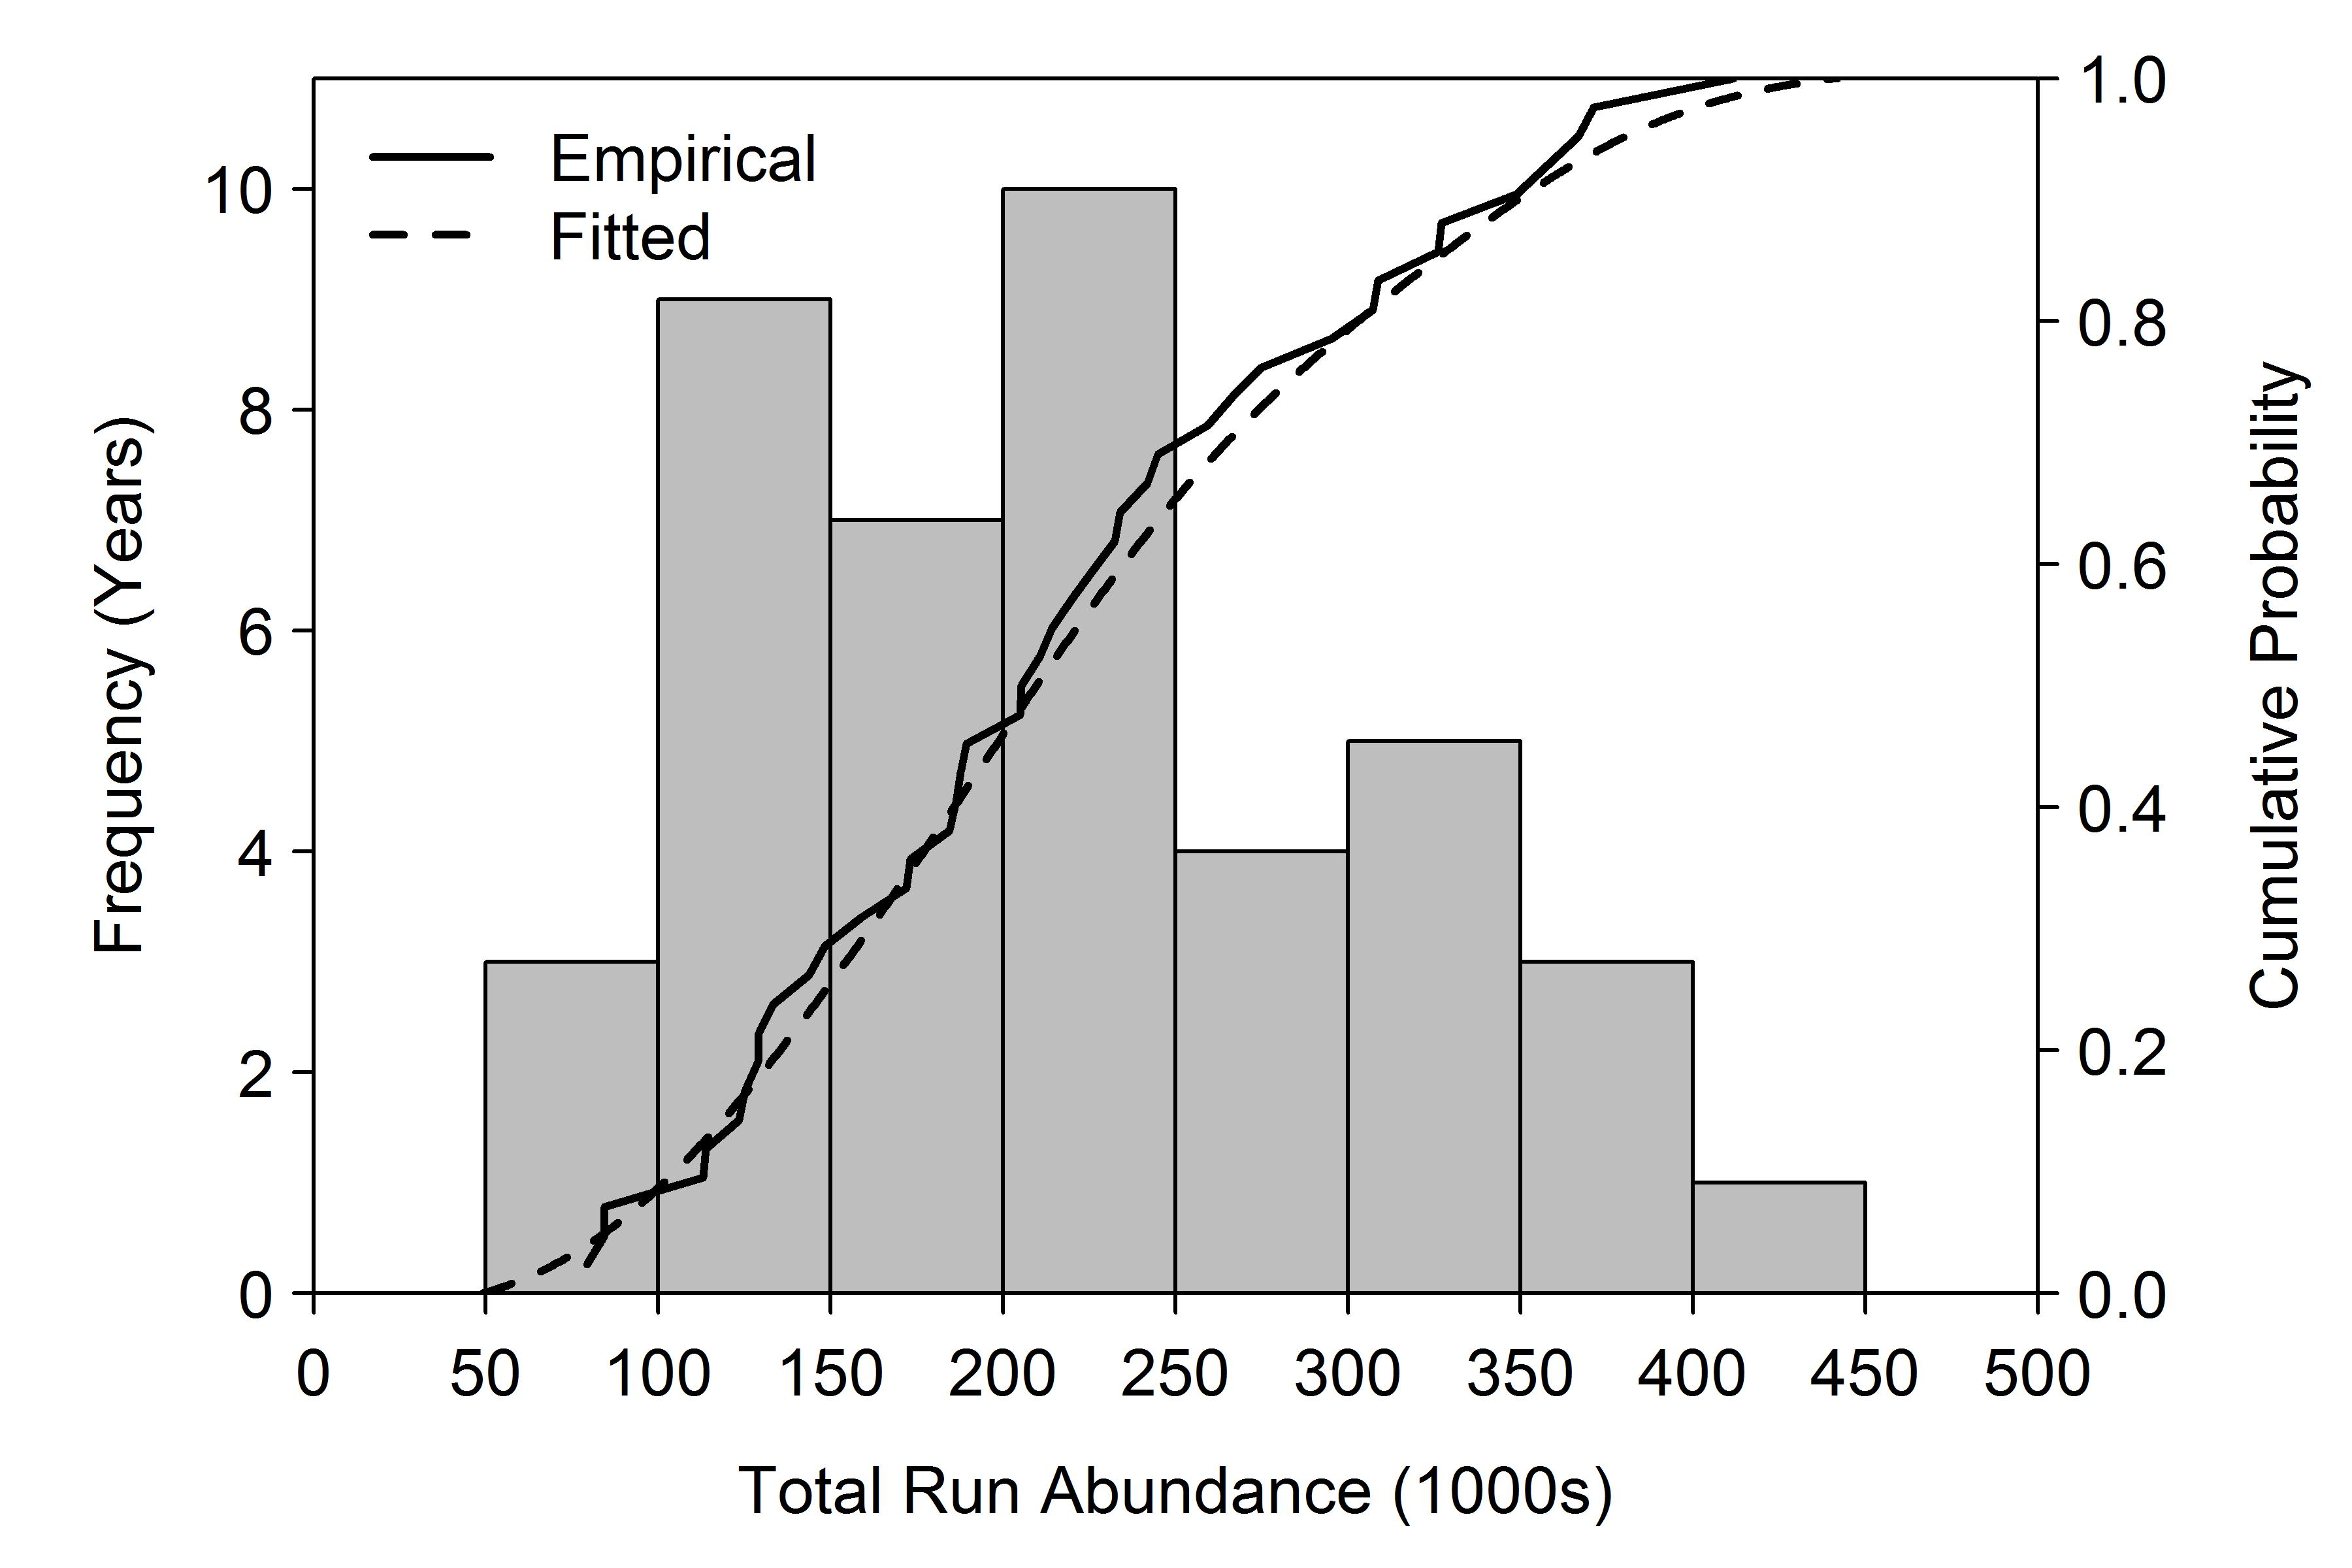
\includegraphics{img/Ch3/N-plot.jpg}
  \caption{Distribution of total drainage-wide run size for Kuskokwim River Chinook salmon, as presented in \cite{liller-etal-2018}. This distribution was used to generate the run size of the aggregate Chinook salmon populations entering the fishery system in a simulated year. The secondary $y$-axis represents the probability of a run falling below a given run size according to the historical frequency of run sizes; where the solid line shows the empirical cumulative distribution function and the dashed line shows one obtained by fitting a kernel density smoother to the empirical data. The fitted distribution was used for simulation to prevent the same 42 run size values from being replicated in the analysis.}
  \label{fig:N-plot}
\end{figure}

\clearpage

\begin{figure}
  \centering
  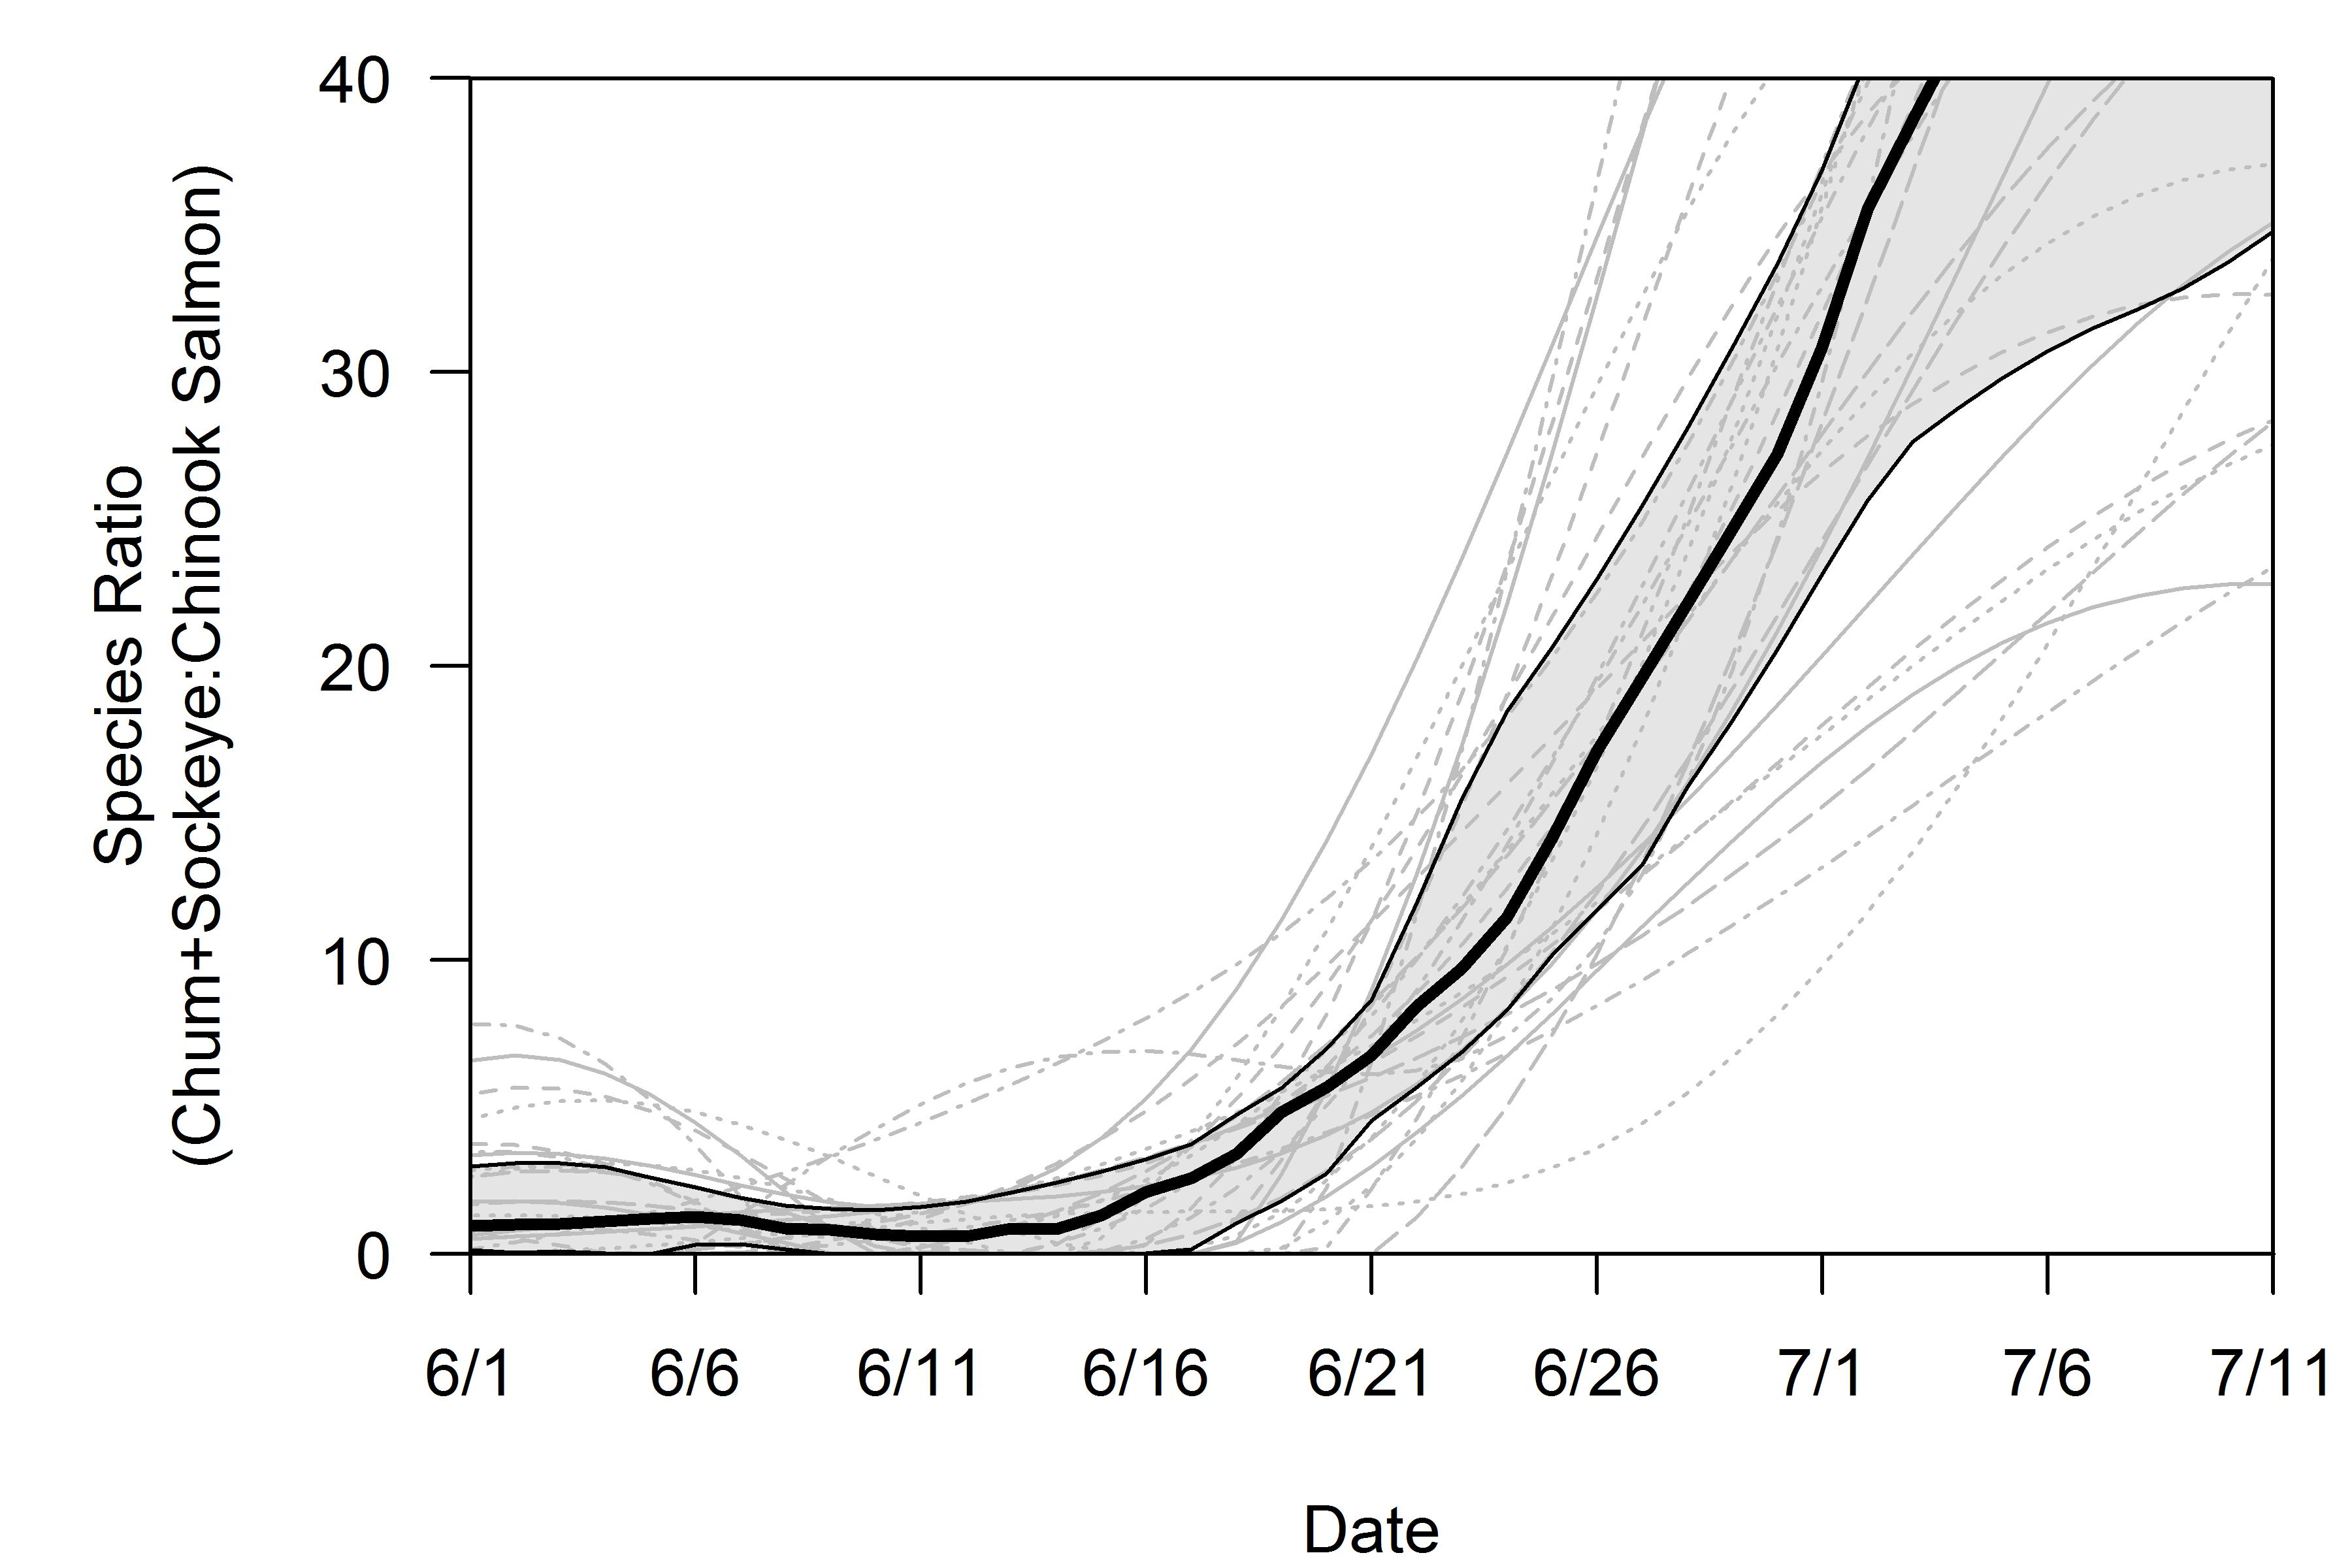
\includegraphics{img/Ch3/ratios-plot.jpg}
  \caption{Smoothed species ratios of chum+sockeye:Chinook salmon as detected by the Bethel Test Fishery. Individual grey lines represent separate years from 1984 -- 2017, the grey region represents the central 50\% of all smoothed ratios on each day and the thick black line represents the daily median. Only this time period is shown because at ratios larger than 20, the differences in the influence of chum/sockeye salmon on Chinook salmon harvest by the subsistence fishery are negligable.}
  \label{fig:ratios-plot}
\end{figure}

\clearpage

\doublespacing

\chapter{Validation of the Operating Model in Chapter
\ref{ch3}}\label{validation-of-the-operating-model-in-chapter-refch3}

For any closed-loop simulation model, the reliability of inferences
drawn will be conditional on the ability of the model components to
capture the important behavioral properties of the real system. Here, I
provide a brief validation that the fishery component of the operating
model does in fact provide a reasonable model of the real system when
the fishery was unrestricted.

First, I thought it important that the model be able to replicate the
relationship between total Chinook salmon run size and total subsistence
salmon harvest. Capturing this pattern was important to ensure that the
fishery would not inadvertently harvest an unrealistically large or
small amount of fish in different run sizes if management mistakes were
made, which would confound my conclusions. As shown in Figure
\ref{fig:HvN}, this historical relationship has been quite noisy for the
observed historical time series, though an increasing pattern has
emerged: in general, more fish have been harvested in years with large
runs than years with small runs. I found that by tuning the catchability
(\(q\)) and effort response coefficients, I was able to reproduce the
pattern and variability quite well.

The next behavior of interest was the spatiotemporal distribution of
harvest. Because in-river salmon fisheries are sequential, fish
harvested in one area are invulnerable to harvest (and escapement) in
upriver areas. It also means that communities in downriver communities
may finish fishing earlier in the season because they are the first to
experience favorable fishing conditions (i.e., high in-river abundance
and resulting catch rates; in the Kuskokwim River drying weather also
plays an important role). If the timing of harvest was not captured
adequately, this would be an indication that the effort response
coefficients were improperly tuned and could result in unrealistic
conclusions. The patterns and variability in the day of the year at
which various percentiles of Chinook salmon harvest was attained by
reach compared between observed data and the modeled outcomes are shown
in Figure \ref{fig:temporal-harvest}. It seems that the patterns and
variability in harvest timing were reasonably well-captured,
particularly for downriver reaches. Reaches 14, 15, 16 and 22 seemed to
have had the largest deviations between observed and modeled patterns,
but given communities in these reaches harvest a negligible amount of
Chinook salmon in comparison to the downriver villages (Figure
\ref{fig:spatial-harvest}), I was not concerned by this finding.

The final important characteristic was the spatial distribution of
end-of-season harvest. Accurately representing this component of the
system would further indicate model adequacy. Figure
\ref{fig:spatial-harvest}) shows a comparison of the proportion of total
drainage-wide Chinook salmon subsistence harvest attributable to
communities in each reach between observed and modeled outcomes. While
the overall pattern was fully captured, there were moderate deviations
between the model and observations in reaches 2, 3, and 4.

\clearpage

\begin{figure}
  \centering
  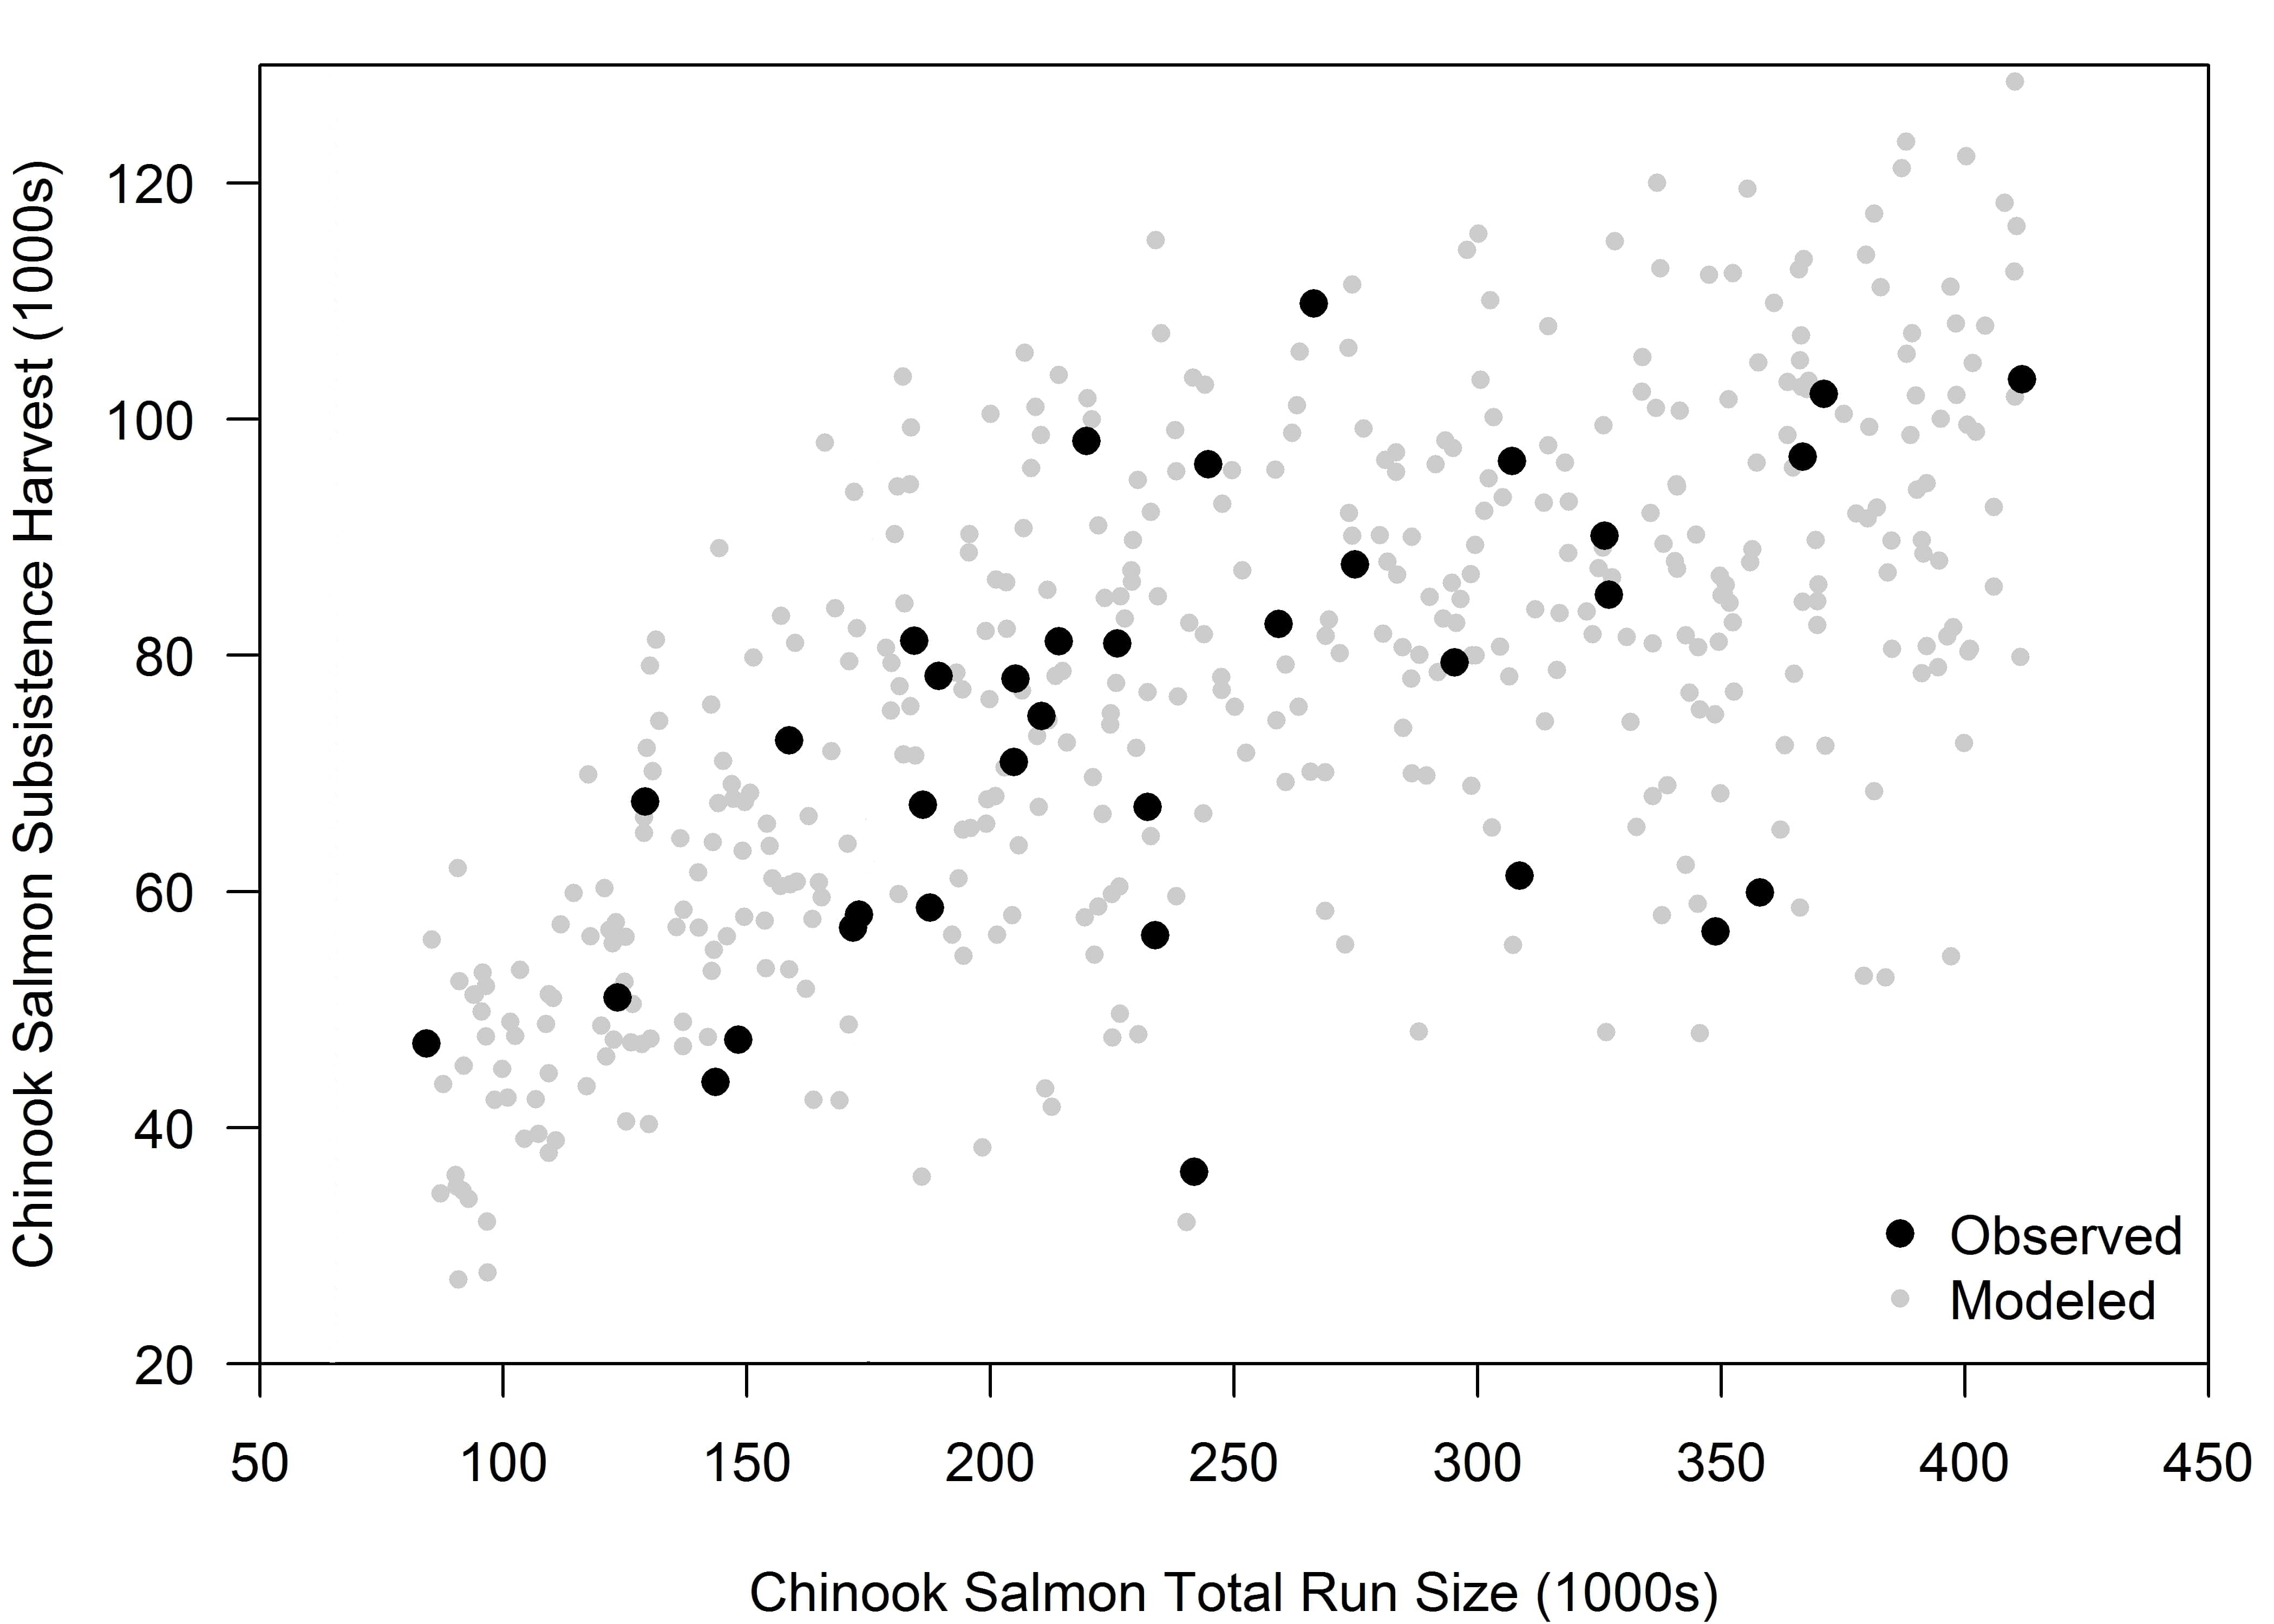
\includegraphics{img/Ch3/FigureB1_noline.jpg}
  \caption{Observed and modeled Chinook salmon subsistence harvest as a function of total Chinook salmon run size. Individual black dots are historical realizations in years with no harvest restrictions on the subsistence salmon fishery. Individual grey dots are modeled outcomes, each representing a hypothetical salmon run with different random subpopulation compositions, run timing, and species ratios.}
  \label{fig:HvN}
\end{figure}

\clearpage

\begin{figure}
  \centering
  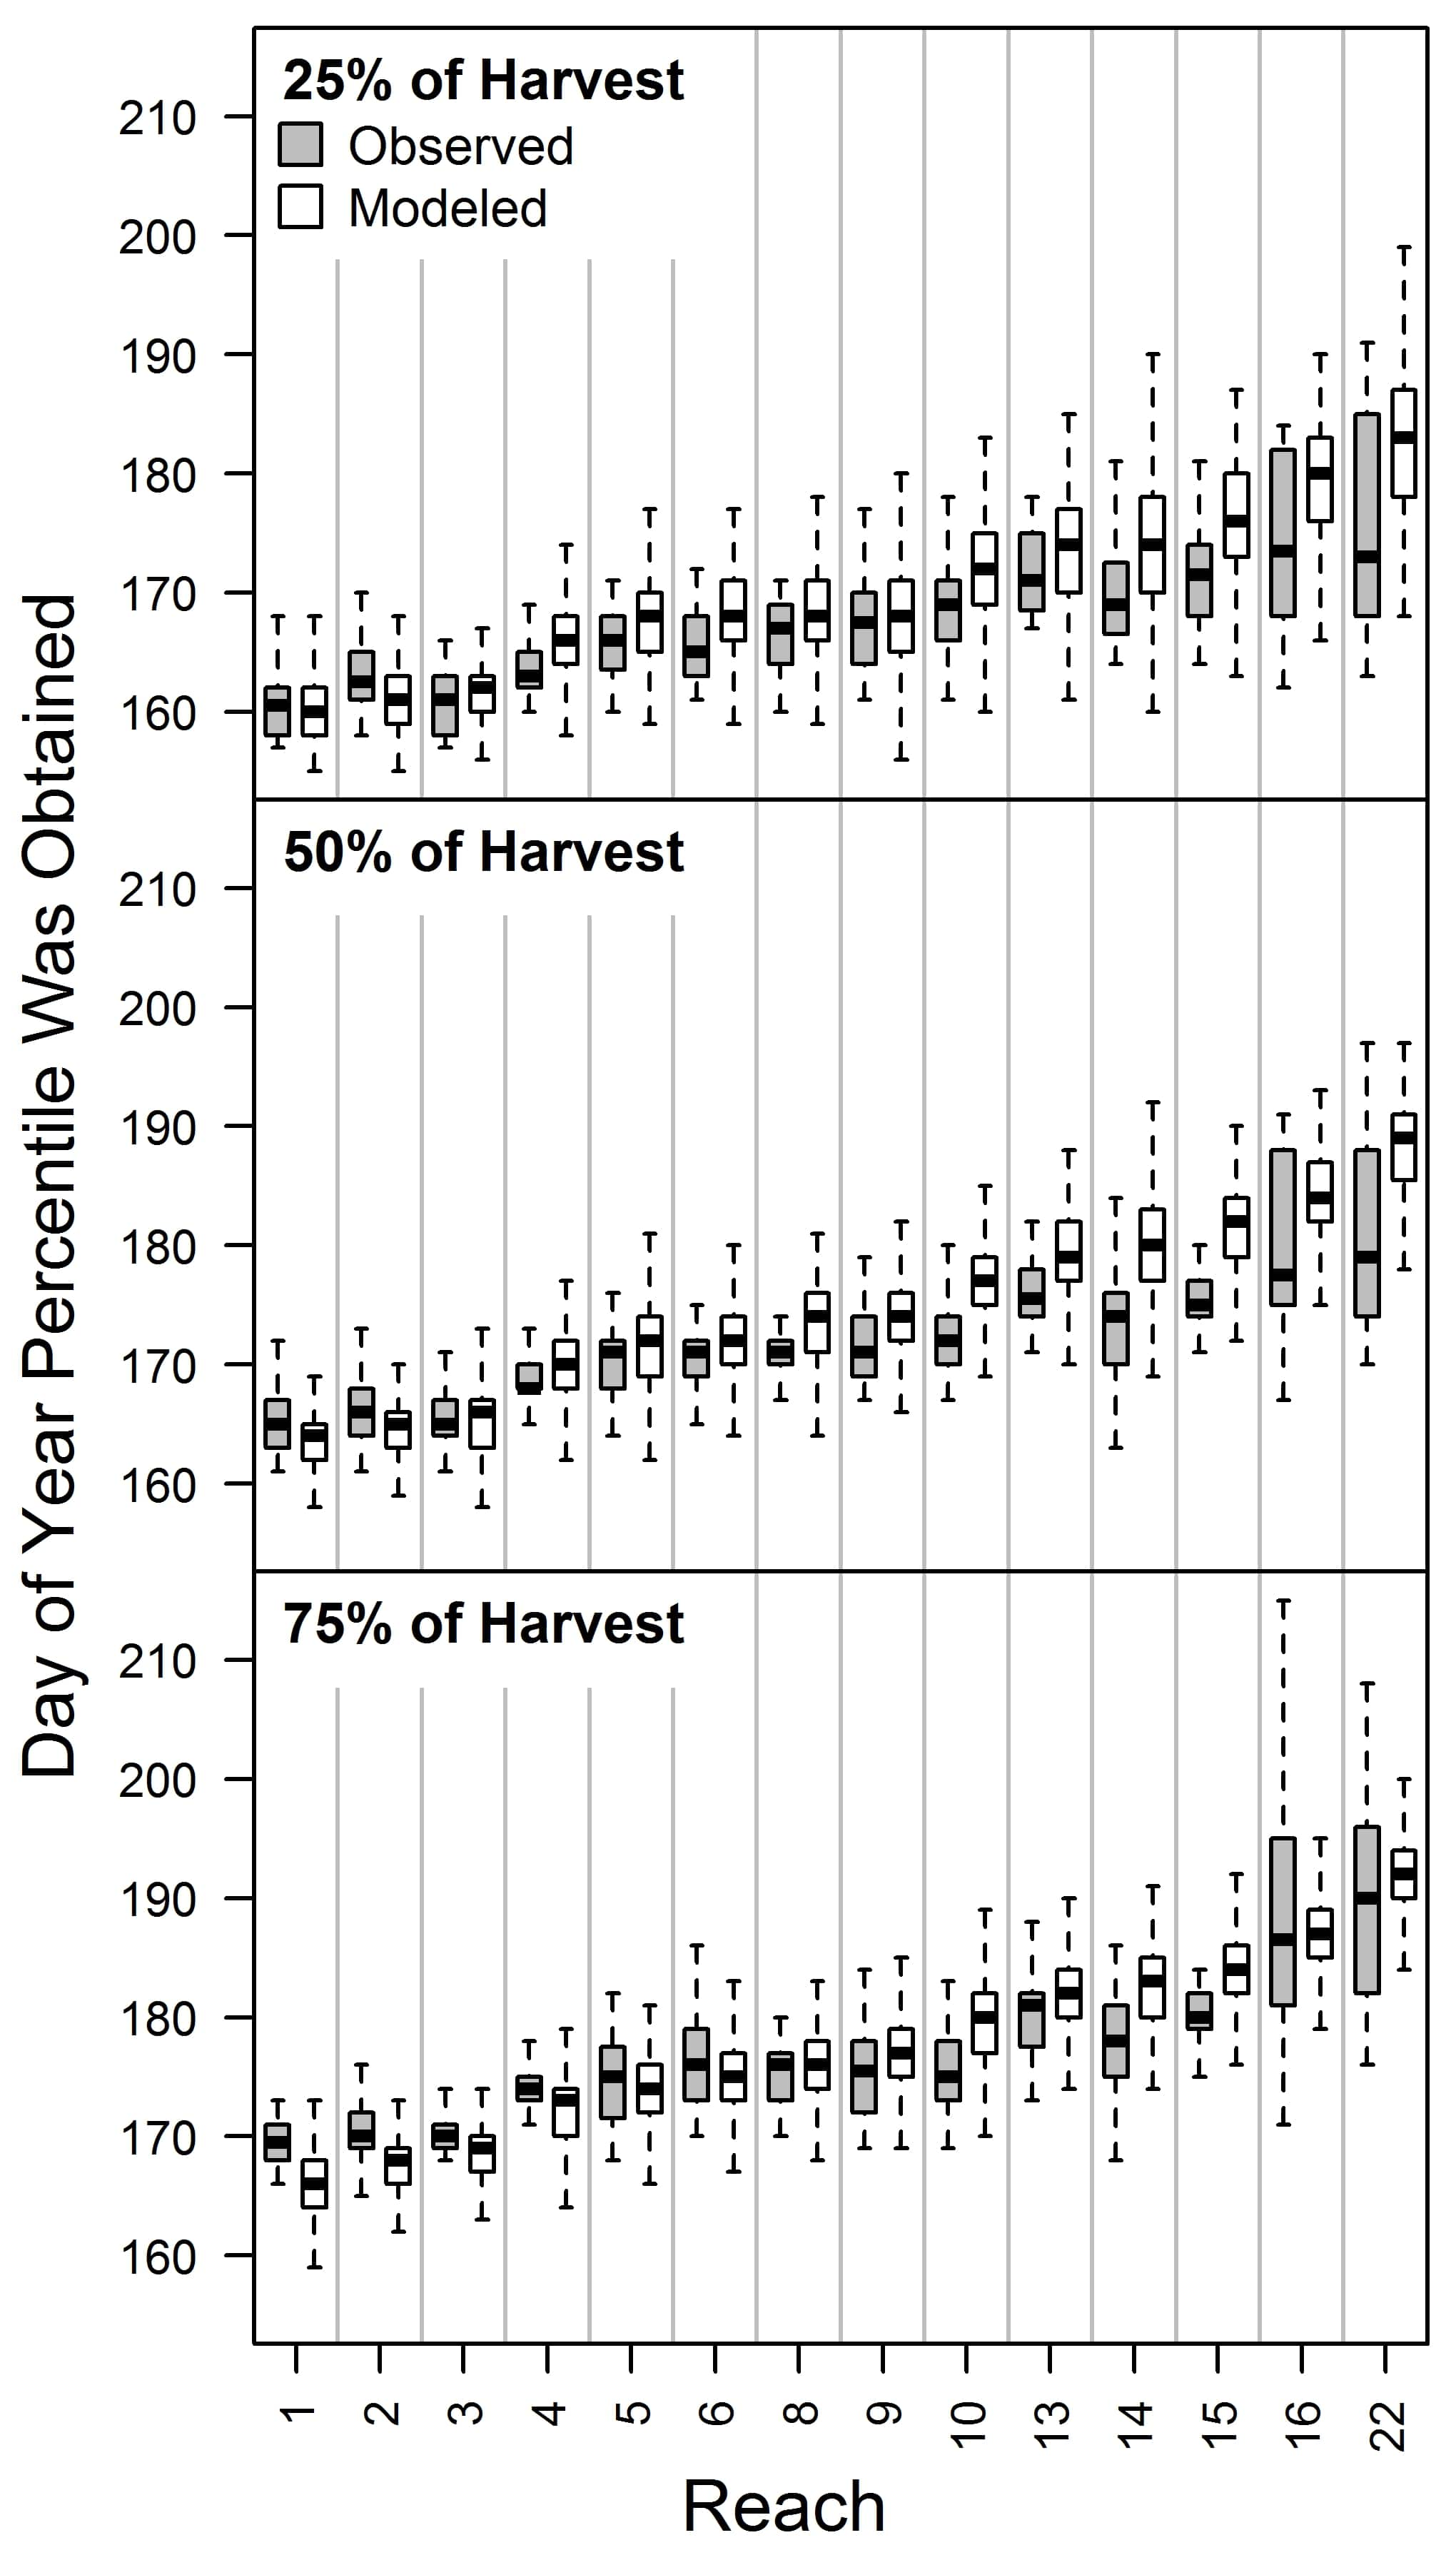
\includegraphics{img/Ch3/FigureB2.jpg}
  \caption{Comparison of the day of the year at which various percentiles of Chinook salmon harvest was attained by reach between observed and modeled outcomes. Variability in the observed boxplots is due to inter-annual variability in run size and timing and represents between-simulation variability for the modeled outcomes. Reach numbers are ordered from downriver to upriver. Note that not all reaches contain communities that harvest salmon.}
  \label{fig:temporal-harvest}
\end{figure}

\clearpage

\begin{figure}
  \centering
  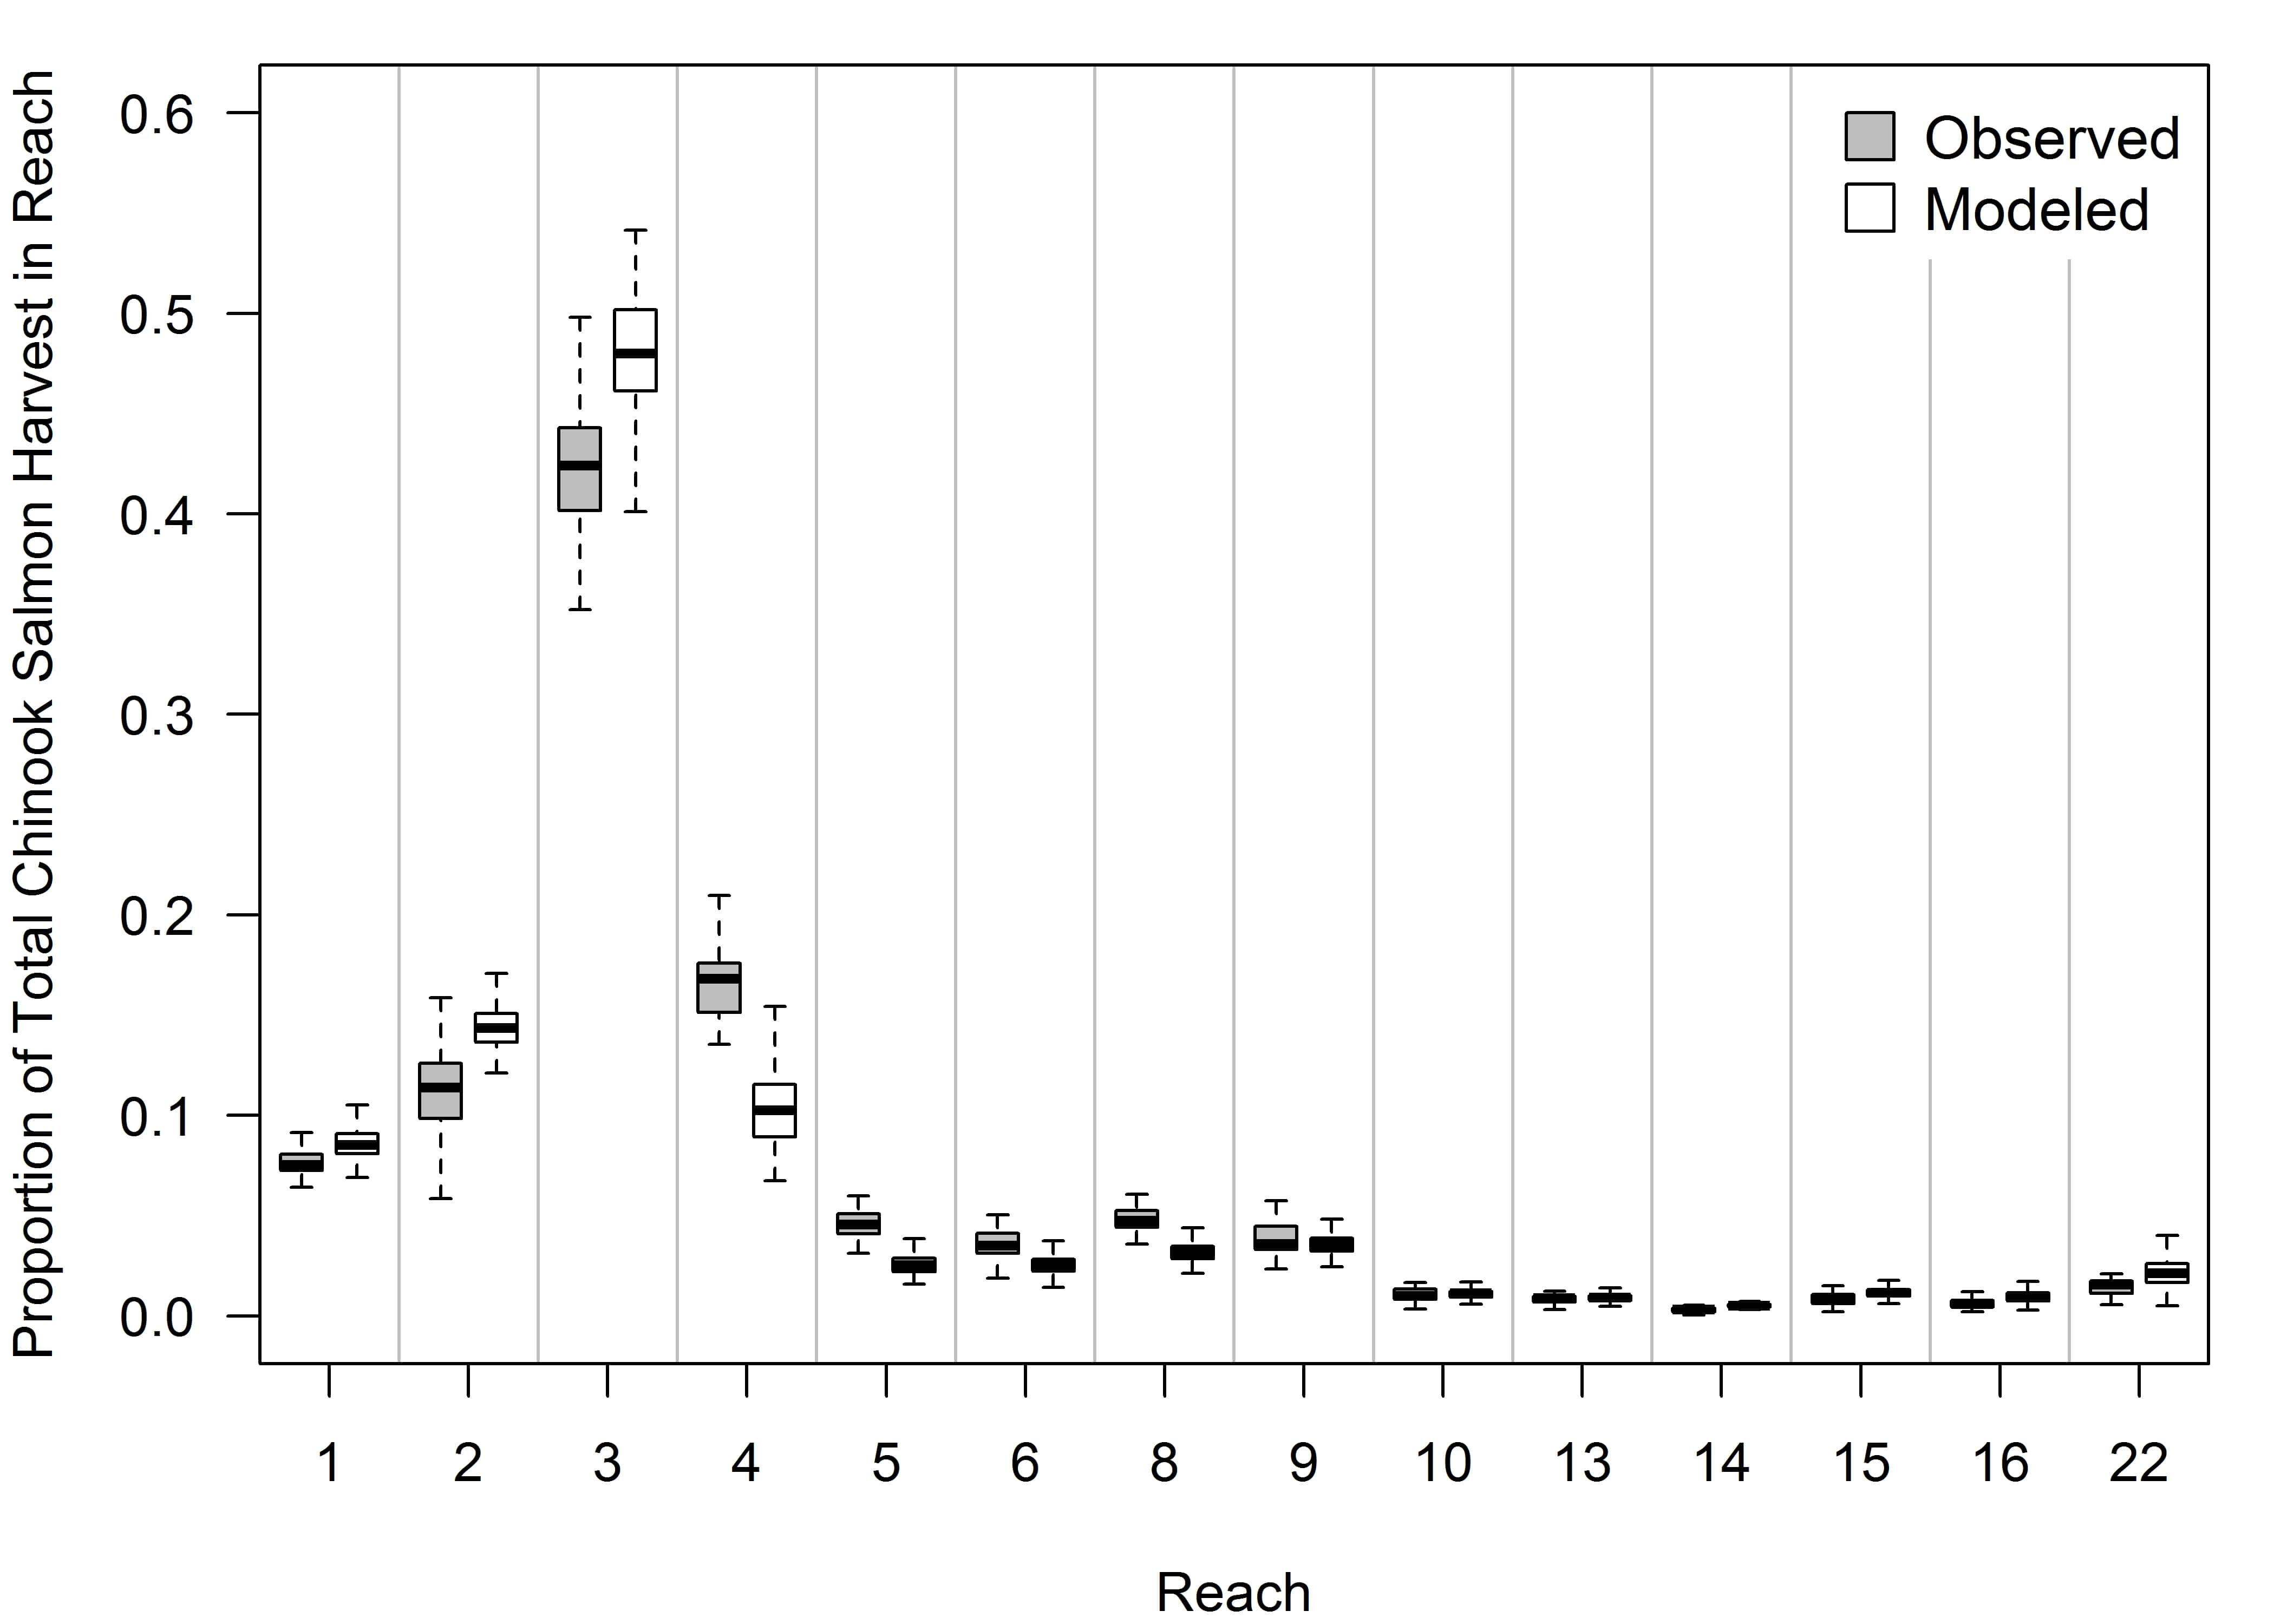
\includegraphics{img/Ch3/FigureB3.jpg}
  \caption{Comparison of the proportion of total drainage-wide Chinook salmon subsistence harvest attributable to communities in each reach between observed and modeled outcomes. Variability in the observed boxplots is due to inter-annual variability, and represents between-simulation variability for the modeled outcomes. Reach numbers are ordered from downriver to upriver. Note that not all reaches contain communities that harvest salmon.}
  \label{fig:spatial-harvest}
\end{figure}

\bibliography{cites-without-doi.bib,cites-with-doi.bib}


\end{document}
